%==============================================================================
% Minor Project -- Mid-Term Evaluation Report
%
%   CausalLine: Influence-Aware Selective Recovery for Multi-Agent LLM Systems
%
% Build:  pdflatex main && bibtex main && pdflatex main && pdflatex main
% See README.md for package requirements and for where each number comes from.
%==============================================================================
% No custom document class and no algorithm package: this builds on a base
% LaTeX installation. Only graphicx, amsmath/amssymb, booktabs and array are
% loaded, all of which ship with every standard distribution (TeX Live
% scheme-basic, MiKTeX basic, Overleaf). The IEEE-like appearance -- two
% columns, Roman section numbers, centred small-caps headings -- is produced
% below with kernel commands rather than by a class file.
\documentclass[10pt,twocolumn,a4paper]{article}

\usepackage[T1]{fontenc}
\usepackage[utf8]{inputenc}
\usepackage{graphicx}
\usepackage{amsmath}
\usepackage{amssymb}
\usepackage{booktabs}
\usepackage{array}

% --- page geometry, set without the geometry package -------------------------
\setlength{\textwidth}{18.0cm}
\setlength{\textheight}{24.7cm}
\setlength{\oddsidemargin}{-0.7cm}
\setlength{\evensidemargin}{-0.7cm}
\setlength{\topmargin}{-1.2cm}
\setlength{\headheight}{12pt}
\setlength{\columnsep}{0.7cm}
\setlength{\parindent}{1em}

% --- IEEE-style sectioning ---------------------------------------------------
\renewcommand{\thesection}{\Roman{section}}
\renewcommand{\thesubsection}{\Alph{subsection}}
\renewcommand{\thesubsubsection}{\arabic{subsubsection})}

\makeatletter
\renewcommand{\section}{\@startsection{section}{1}{\z@}%
  {2.2ex plus 1ex minus .2ex}{1.2ex plus .2ex}%
  {\centering\normalfont\normalsize\scshape}}
\renewcommand{\subsection}{\@startsection{subsection}{2}{\z@}%
  {2.0ex plus 1ex minus .2ex}{1.0ex plus .2ex}%
  {\normalfont\normalsize\itshape}}
\renewcommand{\subsubsection}{\@startsection{subsubsection}{3}{\z@}%
  {1.6ex plus 1ex minus .2ex}{-1em}%
  {\normalfont\normalsize\itshape}}
\makeatother

% --- a hand-rolled algorithm float, so no algorithm package is needed --------
\newcounter{algocount}
\newenvironment{algo}[1]{%
  \begin{figure}[t]%
  \refstepcounter{algocount}%
  \hrule height 0.9pt \vspace{2pt}%
  \noindent\textbf{Algorithm \thealgocount:} #1\par
  \vspace{2pt}\hrule height 0.4pt \vspace{3pt}%
  \footnotesize
  \begin{tabular}{@{}r@{\hspace{0.6em}}p{0.82\columnwidth}@{}}%
}{%
  \end{tabular}\par\vspace{3pt}\hrule height 0.9pt
  \end{figure}%
}
% one algorithm line: \aline{indent level}{text}
\newcommand{\aline}[3]{#1 & \hspace{#2em}#3\\}

\newcommand{\sys}{CausalLine}
\newcommand{\bzero}{B0}
\newcommand{\bone}{B1}
\newcommand{\btwo}{B2}

% Narrow column type for the literature table
\newcolumntype{L}[1]{>{\raggedright\arraybackslash}p{#1}}

\begin{document}

\title{\textbf{\sys{}: Influence-Aware Selective Recovery\\
After Prompt Injection in Multi-Agent LLM Systems}}

\author{
Minor Project Group\\
\normalsize Department of Computer Science and Engineering\\
\normalsize Mid-Term Evaluation, B.Tech.\\
\normalsize Project repository: \texttt{github.com/Siddharthpandey20/CausalLine}
}

\date{}

\maketitle

%==============================================================================
\begin{abstract}
Multi-agent systems built on large language models can be compromised through
prompt injection delivered by a web tool, a shared memory entry, or a message
from another agent. Most existing work addresses \emph{detecting} that a
compromise occurred. This project addresses the step that follows: once a
detector names a malicious source, deciding which completed work must be
recomputed and which may safely be kept. Standard practice discards the
compromised agent's output and everything reachable from it. We implemented
\sys{}, a recovery procedure that records provenance during execution,
establishes per-pair influence using agent self-report together with
counterfactual replay, propagates contamination along only three recorded
relations instead of call-graph reachability, replays only affected events
while splicing the remainder byte-exactly, and verifies the recovered run
before accepting it, escalating to agent restart and then full restart on
failure. The system was evaluated on a purpose-built 56-agent, six-stage,
145-event workflow spanning three inference providers, under three attack
channels and fifteen distinct attack placements. Against the topology-closure
baseline, \sys{} preserved $7.0$ and $15.2$ percentage points more correct work
in the two heavier contamination regimes and lost $17.4$ points in the light
regime, with zero unsafe preservations and zero contamination escapes in all
fifteen runs. It is more expensive in tokens than every baseline, including
full restart, so the report also states the conditions under which it should
not be used.
\end{abstract}

%==============================================================================
\section*{Impact Statement}
Agent frameworks are increasingly used for work that is expensive to repeat:
multi-step research, document pipelines, and tool-using assistants that write
to external systems. When such a pipeline is found to have consumed poisoned
input, the safe response available today is to discard everything downstream of
the compromise. In the workflow studied here that is up to $91\%$ of the
execution trace, of which a measured $76\%$ was actually affected. This project
builds and evaluates machinery that narrows what must be thrown away while
checking its own result before accepting it, so that the cautious option
remains available as a fallback rather than as the only option. The direct
beneficiaries are developers and operators of agent pipelines who need an
incident response more precise than "restart everything". The report is equally
explicit about where the approach costs more than it saves, which is necessary
for anyone deciding whether to adopt it.

%==============================================================================
\vspace{0.6em}
\noindent\textbf{\textit{Index Terms}}---Agent orchestration, Contamination
recovery, Large language models, Multi-agent systems, Prompt injection,
Provenance tracking.
\vspace{0.6em}

%==============================================================================
\section{Introduction}

A multi-agent LLM system is a set of language-model agents that exchange
intermediate results and read from external sources: web pages returned by a
tool, values held in shared memory, and messages produced by other agents. Each
of those channels is a path by which an attacker-controlled instruction can
enter the system, a class of attack established as indirect prompt
injection~\cite{greshake2023,perez2022,liu2024}.

A substantial body of work addresses prevention and detection, either by
hardening the prompt interface~\cite{chen2024} or by tracking how untrusted
content flows through an agent~\cite{neurotaint2026,granularity2026}. This
project begins one step later. We assume the detector has already fired and has
named one or more malicious sources, and we ask the operational question that
follows: of the work the system has already completed, how much must be
recomputed?

The answer used in practice is to discard the output of the compromised agent
and everything reachable from it in the call graph. That rule is safe, simple,
and frequently far too broad, because \emph{reachability is not causation}. An
agent that received a poisoned value in its context may never have used it. In
the workflow we built, a single coordinating agent broadcasts a consolidated
record list to twelve downstream specialists; every specialist is therefore
\emph{exposed} to a poisoned record, while each one actually \emph{uses}
exactly one record. Measured on our testbed, reachability-based recovery
discards up to $91.4\%$ of a $145$-event trace where the genuinely affected
fraction is $76.3\%$.

\textbf{Scope of the claim.} The distinction between a source being present in
a context and a source changing an output is not introduced
here; it is established for LLM agents in prior
work~\cite{neurotaint2026,granularity2026}, as is counterfactual re-execution
as the mechanism for establishing which of the two
occurred~\cite{car2026,causalflow2026}. What this project implements and
evaluates is the recovery procedure built on that distinction: a
detector-triggered, verified selective recomputation with a restart fallback.

\textbf{What was built.} The deliverable is a working Python implementation of
approximately $36{,}000$ lines comprising an execution tracer, a provenance
and influence estimator, a contamination propagation engine, a recovery
planner, a selective replay engine with byte-exact splicing, a verification and
escalation layer, three baselines for comparison, and two evaluation harnesses.
It was exercised on a purpose-built 56-agent workflow running across a local
Llama-3-8B deployment and two hosted providers.

The remainder of the report is organised as follows. Section~\ref{sec:motiv}
explains why the problem was worth addressing and lists the project's
contributions. Section~\ref{sec:lit} reviews related work and identifies the
research gap. Section~\ref{sec:prob} states the problem formally.
Section~\ref{sec:frame} describes the implemented system, including the
56-agent testbed and the algorithms. Section~\ref{sec:exp} reports the
experimental configuration, results and their interpretation.
Section~\ref{sec:concl} concludes and states the planned work.

%==============================================================================
\section{Motivation}
\label{sec:motiv}

Three observations motivated the project.

\textbf{Recovery is coarse because precision is unavailable, not because
coarseness is desired.} Classical taint tracking propagates along
reachability~\cite{newsome2005,king2003} because, in a program, every data
dependency is visible in the instruction stream. In an LLM agent it is not: the
only record of whether a source in the context window changed the output is the
output itself. Recovery is therefore forced to be conservative unless influence
can be established by some other means.

\textbf{The cost of over-discarding grows with system size.} In a four-agent
chain, discarding everything downstream of the first agent costs a few events.
In a fan-out topology with a coordinating hub, the same rule discards almost the
entire trace, because the hub makes every later agent reachable from every
earlier source. Agent frameworks are moving toward exactly these shapes, so the
penalty is increasing rather than shrinking.

\textbf{A recovery that is wrong is worse than one that is wasteful.} If
recovery preserves an event that was in fact contaminated, the attack survives
the incident response. This asymmetry governs every design decision in the
implementation: evidence that \emph{enlarges} the recovery region is accepted
cheaply, while evidence that \emph{shrinks} it must be strong, and anything
unexamined is treated as contaminated.

The 56-agent, three-provider testbed was chosen for the same reason. A
five-agent single-model pipeline cannot exhibit the hub effect that makes the
problem interesting, and cannot show whether provenance survives a contamination
path that crosses providers with different tokenizers and different
instruction-following behaviour.

\subsection{Contributions}

\begin{enumerate}
\item \textbf{An implemented recovery procedure} that consumes a detector's
verdict and produces a minimal recovery set, propagating contamination along
three recorded relations --- influence, derivation and ingestion --- rather
than call-graph reachability (Section~\ref{sec:prop}).

\item \textbf{An influence estimator with an explicit soundness discipline},
combining agent self-report with counterfactual replay, treating positive and
negative evidence asymmetrically, and treating every unexamined pair as
contaminated (Section~\ref{sec:attrib}).

\item \textbf{A verification and escalation layer} that refuses to accept a
recovered run until a task-level check, a live-memory check and a redaction
check all pass, escalating selective $\rightarrow$ agent restart $\rightarrow$
full restart on failure (Section~\ref{sec:verify}).

\item \textbf{A 56-agent, six-stage, three-provider evaluation testbed} with
three independent attack channels and a seed-driven attack placement generator
(Section~\ref{sec:testbed}).

\item \textbf{A measured comparison against three baselines} over fifteen runs
with fifteen distinct attack placements, plus a deterministic scripted matrix of
$96$ cells $\times\,30$ repetitions under four detectors
(Section~\ref{sec:exp}).

\item \textbf{A diagnosed and corrected provenance defect.} A missing relation
in the contamination walk caused five events holding attacker-controlled text
to be preserved; the defect first presented as a $+17.2$-point apparent
improvement (Section~\ref{sec:defect}).
\end{enumerate}

%==============================================================================
\section{Literature Work}
\label{sec:lit}

\subsection{Attack surface and detection}
Indirect prompt injection against LLM-integrated applications was characterised
by Greshake et al.~\cite{greshake2023}, who demonstrated delivery through
retrieved content rather than direct user input. Perez and
Ribeiro~\cite{perez2022} catalogued instruction-override techniques, and Liu et
al.~\cite{liu2024} contributed a formalisation and benchmark for attacks and
defences. Chen et al.~\cite{chen2024} defend by separating instructions from
data at the prompt interface. All of this work is upstream of ours: it aims to
stop or notice the attack, not to repair a system that has already run.

\subsection{Information-flow tracking for LLM agents}
Dynamic taint analysis~\cite{newsome2005} and intrusion
backtracking~\cite{king2003} established reachability-based propagation for
conventional software. NeuroTaint~\cite{neurotaint2026} argues this transfers
poorly to LLM agents, because propagation there is governed by probabilistic
natural-language reasoning rather than explicit memory writes, and must model
semantic transformation and causal influence on decisions; it is evaluated
across a 400-scenario benchmark spanning 20 agent frameworks. Fan et
al.~\cite{granularity2026} track provenance at the granularity of individual
tool arguments and use it to reject tainted arguments before a tool executes.
Both separate exposure from influence, and both apply it to
detection or enforcement rather than to repair.

\subsection{Counterfactual attribution}
Causal Agent Replay~\cite{car2026} models an agent run as a structural causal
model, intervenes on a step, re-executes forward, and measures the shift in the
outcome distribution. CausalFlow~\cite{causalflow2026} computes step-level
causal responsibility by intervention and synthesises minimal repairs that flip
a failure into a success. Our influence estimator belongs to this family; we
claim no novelty for the mechanism itself.

\subsection{Contamination, debugging and replay economics}
Mazhar et al.~\cite{tracelevel2026} measure contamination in multi-agent traces
by injecting perturbations and observing trace divergence, reporting that
structural divergence and outcome corruption are decoupled.
DoVer~\cite{dover2026} checkpoints each step, intervenes on a message and
resumes, for hypothesis-driven debugging. Kang et al.~\cite{zeroreplay2026}
compile traces into event knowledge graphs and predict where a scarce replay
budget should be spent, explicitly aiming to avoid paying for counterfactual
replay. The survey of Wang et al.~\cite{trustsurvey2026} places recovery among
the trust functions built on execution provenance, populating it with
retry-based repair, transactional compensation and checkpoint-restore, and notes
that rollback can itself produce semantically unsafe re-executions.
Checkpoint-and-rollback is long established in message-passing
systems~\cite{elnozahy2002}.

\subsection{Comparative analysis}

Table~\ref{tab:lit} compares the most directly relevant work. In the
\textit{Database Used} column, "N/A" indicates the work does not evaluate
against a named dataset or benchmark; \textit{Working Devices} is "N/A"
throughout because none of these are hardware-coupled systems.

\begin{table*}[t]
\centering
\caption{Comparative analysis of related work. The final column states the
limitation or observation relevant to this project.}
\label{tab:lit}
\footnotesize
\setlength{\tabcolsep}{4pt}
\begin{tabular}{L{0.9cm} L{2.6cm} L{2.4cm} L{2.9cm} L{5.4cm} L{1.0cm}}
\toprule
\textbf{Ref.} & \textbf{Technique Used} & \textbf{Database Used} &
\textbf{Accuracy / Measures} & \textbf{Remarks} & \textbf{Working Devices}\\
\midrule

\cite{greshake2023} & Indirect prompt injection via retrieved content &
Case studies on LLM-integrated apps & Qualitative demonstrations &
Establishes the threat and its delivery channels. Does not address what to do
with work already produced under compromise. & N/A \\

\cite{liu2024} & Formalisation and benchmark of injection attacks/defences &
Purpose-built benchmark & Attack success rate & Evaluates prevention and
detection. Recovery after a successful attack is out of scope. & N/A \\

\cite{chen2024} & Structured queries separating instruction from data &
Standard instruction datasets & Attack success rate, utility &
Prevention at the prompt interface. Assumes the defence holds; offers nothing
once it has not. & N/A \\

\cite{neurotaint2026} & Semantic taint tracking for LLM agents (NeuroTaint) &
TaintBench (400 scenarios, 20 frameworks); InjecAgent; ToolEmu &
Source-to-sink propagation detection vs.\ an IFC baseline &
Establishes exposure~$\neq$~influence for LLM agents, which this project
assumes rather than claims. Oriented to offline auditing and detection, not to
selecting work for recomputation. & N/A \\

\cite{granularity2026} & Argument-level provenance for enforcement &
N/A & Enforcement coverage &
Separates exposure from influence per tool argument, but acts \emph{before}
execution by rejecting tainted arguments. No notion of repairing a completed
run. & N/A \\

\cite{car2026} & Structural causal model; do-intervention; Shapley credit &
Synthetic models with known ground truth &
Recovery of pivotal steps and two-step interactions &
Attributes capability failures to steps. No adversary, and no safety
obligation: a wrong attribution costs accuracy, not containment. & N/A \\

\cite{causalflow2026} & Causal responsibility scores; counterfactual repair &
GSM8K; MBPP; SealQA Hard; MedBrowseComp &
$42.7\%$ of failures converted to validated repairs &
Closest published work to "recovery", but single-agent capability repair with
no adversarial model, no contamination propagation and no verification
gate. & N/A \\

\cite{tracelevel2026} & Perturbation injection; trace-divergence measurement &
32 GAIA tasks, 3 models (614 paired runs) &
Divergence and outcome-corruption rates &
Characterises contamination under \emph{natural} noise and measures rather
than repairs. Authors list provenance-based origin attribution as future
work. Its decoupling finding motivates our separate reporting of payload
landing. & N/A \\

\cite{dover2026} & Checkpoint, intervene on a message, resume (DoVer) &
Magentic-One; AutoGen2 MathChat &
Debugging success on failure hypotheses &
Mechanically the closest to our checkpoint-and-splice layer, but aimed at
debugging general failures; no contamination model and no verification
obligation. & N/A \\

\cite{zeroreplay2026} & Event knowledge graph; predict high-impact events &
Held-out trace families &
Branch Recall@5 $=0.93$ (baseline $0.73$) &
Attacks the same cost problem from the opposite direction, by avoiding replay
rather than justifying it. Complementary to our economic analysis. & N/A \\

\cite{trustsurvey2026} & Survey of execution provenance as a trust substrate &
N/A & N/A &
Places recovery in its taxonomy, populated with retry, compensation and
rollback, and observes that rollback can yield semantically unsafe
re-executions --- the hazard our verification layer targets. & N/A \\

\cite{newsome2005}, \cite{king2003} & Dynamic taint analysis; intrusion
backtracking & Commodity binaries; OS-level logs &
Detection and dependency-graph reduction &
Reachability-based propagation, which is precisely our \btwo{} baseline.
Assumes deterministic, observable data dependencies that LLM agents do not
provide. & N/A \\

\bottomrule
\end{tabular}
\end{table*}

\subsection{Research gap}

The reviewed work establishes four things we build on: that the attack is
real~\cite{greshake2023,liu2024}; that exposure is not influence in LLM
agents~\cite{neurotaint2026,granularity2026}; that counterfactual re-execution
can establish which of the two occurred~\cite{car2026,causalflow2026}; and that
contamination in multi-agent traces is measurable~\cite{tracelevel2026}.

The gap is operational and has three parts.

\emph{First}, existing influence tracking is aimed at detection or enforcement.
It answers "did untrusted data reach a sink", not "which of the artefacts this
system already produced may be kept".

\emph{Second}, the attribution work targets capability failures under no
adversary~\cite{car2026,causalflow2026}. Such a system has no safety
obligation: an incorrect attribution costs accuracy. In the adversarial setting
an incorrect attribution preserves an attack, which demands the asymmetric
evidence discipline described in Section~\ref{sec:attrib}.

\emph{Third}, where recovery does appear it is retry, compensation or
rollback~\cite{trustsurvey2026}, and the same survey notes that rollback can
produce semantically unsafe re-executions. We found no published system that is
triggered by a detector's verdict on a malicious source, restricts propagation
below reachability, and gates its output on verification before accepting it.

This project addresses that combination. It does not claim to introduce the
underlying distinction or the attribution mechanism.

%==============================================================================
\section{Problem Definition}
\label{sec:prob}

Let a completed run be a trace $T=(E,S)$ where $E$ is a sequence of recorded
events and $S$ a set of sources. Each event $e \in E$ carries its exposures
$X(e)\subseteq S$, the sources present in its agent's context. A detector
supplies a flagged set $M \subseteq S$ of malicious sources.

\textbf{Input:} the trace $T$, the flagged set $M$, and the stored prompts,
outputs and checkpoints of the run.

\textbf{Desired output:} an invalidation set $I \subseteq E$ to recompute, such
that the recovered run is free of attacker influence and $|I|$ is as small as
the available evidence allows.

Let $C(M) \subseteq E$ be the set of events truly influenced by $M$. The
requirement is a safety constraint, not an objective to trade away:
\begin{equation}
C(M) \subseteq I
\label{eq:safety}
\end{equation}
Any $e \in C(M)\setminus I$ is an \emph{unsafe preservation}: recovery kept an
event the attacker influenced. Subject to~\eqref{eq:safety}, the objective is
\begin{equation}
\min_{I} \; |I| \quad\text{equivalently}\quad
\max_{I} \; \textit{work preserved} = 1 - \frac{|I|}{|E|}
\label{eq:objective}
\end{equation}

\textbf{Constraint.} $C(M)$ is not observable at recovery time; only exposure
is recorded. Influence must be estimated, and the estimate
$\hat{C}(M)$ must satisfy $C(M)\subseteq\hat{C}(M)$ to preserve
\eqref{eq:safety}.

\textbf{Existing limitation.} The reachability baseline sets
$I = \mathrm{desc}(M)$, every event downstream of where a flagged source
entered. This satisfies~\eqref{eq:safety} but maximises $|I|$.

\textbf{Objective of this system.} Produce $\hat{C}(M)$ narrower than
$\mathrm{desc}(M)$, improving~\eqref{eq:objective} while never
violating~\eqref{eq:safety}, and verify the recovered run before accepting it.

%==============================================================================
\section{Proposed Framework}
\label{sec:frame}

\subsection{Overall architecture}

\begin{figure*}[t]
\centering
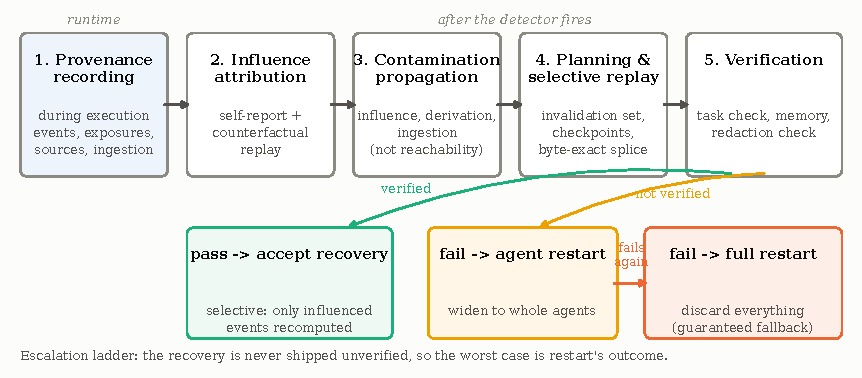
\includegraphics[width=\textwidth]{figures/fig_architecture.pdf}
\caption{The implemented recovery pipeline. Stage~1 runs during the workflow
and is the only stage that costs anything when no attack occurs; stages~2--5
run after a detector names a malicious source. The escalation ladder at the
bottom is what makes the procedure safe to deploy: a recovered run is never
accepted until verification passes, and failure widens the recovery rather than
shipping an unverified result, so the worst case is a full restart's outcome.}
\label{fig:arch}
\end{figure*}

Figure~\ref{fig:arch} shows the five implemented stages. Only stage~1 executes
during the workflow itself.

\subsubsection{Provenance recording}
Every operation is logged as an event carrying its agent, its parent events,
the identifiers of all sources in the agent's context, and a content-addressed
reference to what it produced. Prompts and outputs are stored so that a
counterfactual can be re-issued later. Two record types are written with no
model in the loop because the answer is a property of the code path: a
\emph{structural} record for operations our own code computes, and a
\emph{carrier} record for an event whose output is a copy of an earlier event's,
which inherits that event's verdicts rather than asserting its own. A third,
\emph{ingestion}, records that an event's stored output embeds the content of a
source it retrieved; Section~\ref{sec:defect} explains why it exists.

\subsubsection{Influence attribution}
\label{sec:attrib}
For each (source, event) pair the estimator returns \textit{influenced},
\textit{clean} or \textit{unchecked}. Two mechanisms are combined. Self-report
asks the agent which inputs changed its output; it is cheap and is not trusted
symmetrically. Counterfactual replay re-issues the stored prompt with the source
redacted and compares outputs; this is evidence.

The asymmetry is the safety property. A \textit{tainted} verdict enlarges the
recovery region and is therefore sound to accept on weak evidence, so a
self-report positive is accepted. A \textit{clean} verdict shrinks the region
and requires strong evidence, so a self-report negative is only a hypothesis
until a counterfactual confirms it. Anything unchecked is treated as
contaminated. The implementation additionally checks \emph{removability}: if
redacting a source does not actually remove its information from the prompt
(because another source carries the same fact), the leave-one-out test is void
and the pair stays contaminated.

\subsubsection{Contamination propagation}
\label{sec:prop}
Contamination walks exactly three relations, given in
Algorithm~\ref{alg:contaminate}: influence (source $\rightarrow$ event),
derivation (event $\rightarrow$ the source wrapping its output for a downstream
agent), and ingestion (source $\rightarrow$ the event that retrieved it). It
never walks parent edges, because those record execution order rather than data
dependence; walking them transitively reproduces the \btwo{} baseline exactly.

\subsubsection{Planning and selective replay}
The planner computes the invalidation set and the nearest trusted checkpoint
per agent. Replay re-executes only invalidated events and splices every other
event from its logged output. Two invariants are asserted at run time: every
spliced event's output must match its original log entry, and no model call may
be issued for an event outside the invalidation set. Flagged sources are
redacted from re-issued prompts, and a redaction that cannot be completed
aborts the recovery rather than producing a run that reports a removal which
did not happen.

\subsubsection{Verification and escalation}
\label{sec:verify}
A recovered run is checked before acceptance: the task-level outcome must hold,
no live memory entry may still point at an invalidated write, and no flagged
source may remain in any re-issued prompt. On failure the recovery escalates
selective $\rightarrow$ agent restart $\rightarrow$ full restart. Restart is
therefore never the primary action and always the guaranteed fallback, which
makes "no worse than restart in outcome" a structural property rather than an
empirical observation.

\subsection{The 56-agent evaluation testbed}
\label{sec:testbed}

\begin{figure*}[t]
\centering
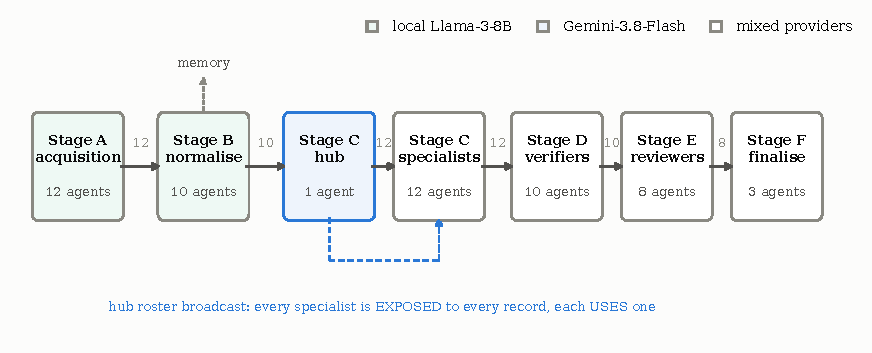
\includegraphics[width=\textwidth]{figures/fig_agent_workflow.pdf}
\caption{Stage-level view of the implemented workflow. Numbers on the arrows
are the agent-to-agent control edges actually recorded in an executed trace.
The dashed return path is the structural point of the design: the hub
broadcasts a consolidated roster, so every specialist is exposed to every
record while each uses exactly one. The dashed upward arrow at Stage~B marks
the memory channel, which has no call-graph edge back to whichever agent wrote
the entry.}
\label{fig:workflow}
\end{figure*}

\begin{figure*}[t]
\centering
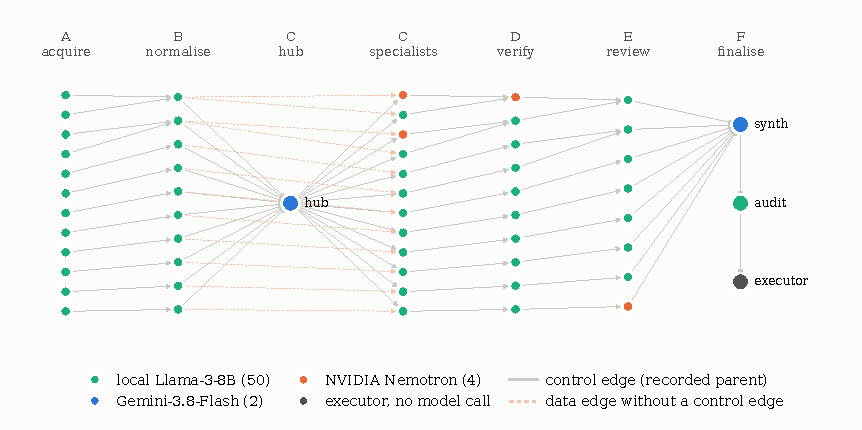
\includegraphics[width=\textwidth]{figures/fig_agent_trace.pdf}
\caption{Agent invocation graph of all 56 agents, derived from a recorded
execution trace rather than from source inspection. Solid edges are control
edges recovered from each event's logged parents; dashed edges are data
dependencies that have no corresponding control edge, which is why
reachability over the call graph alone is not a sound basis for recovery.
Node colour gives the inference provider that answered for that agent.}
\label{fig:trace}
\end{figure*}

Prior measurements in this project used a four-to-five agent chain, which
cannot exhibit the hub effect. We therefore built a larger workflow, summarised
in Table~\ref{tab:topology} and drawn in Figures~\ref{fig:workflow}
and~\ref{fig:trace}. Both figures are generated from
\texttt{diagrams/topology.json}, which is produced by executing the pipeline and
reading the resulting trace, so the edges shown are recorded rather than
asserted.

\begin{table}[t]
\centering
\caption{Implemented workflow. Agent and event counts are read from an executed
trace; the trace contains 145 events and 89 sources in total.}
\label{tab:topology}
\footnotesize
\begin{tabular}{llrr}
\toprule
\textbf{Stage} & \textbf{Role} & \textbf{Agents} & \textbf{Events}\\
\midrule
A & Acquisition (one record each)      & 12 & 48\\
B & Normalisation (memory + a block of A) & 10 & 30\\
C & Hub (fan-in over B, then broadcast) & 1  & 2\\
C & Specialists (roster + one B block)  & 12 & 24\\
D & Verifiers (a block of specialists)  & 10 & 20\\
E & Reviewers (a block of D)            & 8  & 16\\
F & Synthesis / Audit / Executor        & 3  & 5\\
\midrule
  & \textbf{Total}                      & \textbf{56} & \textbf{145}\\
\bottomrule
\end{tabular}
\end{table}

\textbf{Who calls whom.} The recorded control edges follow the pattern
$\mathrm{acq}_i \rightarrow \mathrm{norm}_j$ (12 edges),
$\mathrm{norm}_j \rightarrow \mathrm{hub}$ (10),
$\mathrm{hub} \rightarrow \mathrm{spec}_k$ (12),
$\mathrm{spec}_k \rightarrow \mathrm{ver}_v$ (12),
$\mathrm{ver}_v \rightarrow \mathrm{rev}_r$ (10),
$\mathrm{rev}_r \rightarrow \mathrm{synth}$ (8),
$\mathrm{synth} \rightarrow \mathrm{audit} \rightarrow \mathrm{executor}$, for
66 control edges in total. The data-dependency graph contains 78 edges: the
same 66 plus twelve $\mathrm{norm}_j \rightarrow \mathrm{spec}_k$ edges, where a
specialist reads its own normaliser's record directly in addition to the hub
roster. The executor performs no model call; it compares the final consolidated
list against the known-correct values, so task success never depends on a model
judging its own output.

\textbf{Provider assignment.} Of the 56 agents, 50 run on a local Llama-3-8B
deployment, 2 on \texttt{gemini-3.8-flash} (the two fan-in points, hub and
synthesis), and 4 on an NVIDIA Nemotron endpoint (specialists 1 and 3, verifier
1, reviewer 8). The resulting web-channel contamination path crosses local
$\rightarrow$ Gemini $\rightarrow$ NVIDIA $\rightarrow$ local.

\textbf{Attack channels.} Three channels are implemented, chosen because they
propagate differently: a \emph{web/tool} note planted beside a fetched record,
which arrives through a tool call and therefore has an origin event; a
\emph{poisoned memory} policy entry read at Stage~B, which has no call-graph
edge back to whichever agent wrote it; and an \emph{inter-agent message}
planted into a verifier's context with no derivation link, so it is not the
output of any event in the run.

\textbf{Ground truth.} Each payload instructs the receiving agent to emit a
specific wrong access code, and that code is a canary absent from the corpus. If
it appears in an output, that output was influenced. When a model ignores the
instruction the run is recorded as \texttt{payload\_landed: false} and its
safety counts are reported as arithmetic rather than evidence.

\subsection{Algorithms}

Algorithm~\ref{alg:contaminate} is the propagation engine and
Algorithm~\ref{alg:recover} the end-to-end procedure. Both correspond directly
to \texttt{src/provenance/contamination.py} and \texttt{src/recovery/}.

\begin{algo}{Contamination propagation}
\label{alg:contaminate}
\aline{}{0}{\textbf{Input:} trace $T=(E,S)$, flagged sources $M$,}
\aline{}{1.4}{cleared pairs $K$}
\aline{}{0}{\textbf{Output:} contaminated event set $\hat{C}$}
\aline{1}{0}{$\hat{C} \gets \emptyset$;\ \ $B \gets \emptyset$;\ \ $Q \gets M$}
\aline{2}{0}{\textbf{while} $Q \neq \emptyset$ \textbf{do}}
\aline{3}{1}{pop $s$ from $Q$}
\aline{4}{1}{\textbf{if} $s \in B$ \textbf{then continue}}
\aline{5}{1}{$B \gets B \cup \{s\}$}
\aline{6}{1}{\textbf{for} each $e$ with an influence or ingestion}
\aline{}{2.4}{edge from $s$ \textbf{do}}
\aline{7}{2}{$\hat{C} \gets \hat{C} \cup \{e\}$\ \ \textit{// established}}
\aline{8}{1}{\textbf{for} each $e$ with $s \in X(e)$,
             $(s,e) \notin K$ \textbf{do}}
\aline{9}{2}{$\hat{C} \gets \hat{C} \cup \{e\}$}
\aline{}{2}{\textit{// unchecked exposure is assumed}}
\aline{}{2}{\textit{// to be influence}}
\aline{10}{1}{\textbf{for} each $e \in \hat{C}$ and $s'$ with}
\aline{}{2.4}{$\mathrm{derivedFrom}(s')=e$ \textbf{do}}
\aline{11}{2}{$Q \gets Q \cup \{s'\}$}
\aline{}{2}{\textit{// cross the agent boundary}}
\aline{12}{0}{\textbf{return} $\hat{C}$}
\end{algo}

\begin{algo}{Detector-triggered verified recovery}
\label{alg:recover}
\aline{}{0}{\textbf{Input:} trace $T$, flagged sources $M$}
\aline{}{0}{\textbf{Output:} accepted recovered run, or a full restart}
\aline{1}{0}{establish influence for pairs reachable from $M$}
\aline{}{0}{\textit{// self-report first, then counterfactual}}
\aline{2}{0}{$\mathit{scope} \gets \textsc{Selective}$}
\aline{3}{0}{\textbf{for} $\mathit{attempt} = 1 \ldots 3$ \textbf{do}}
\aline{4}{1}{$I \gets \textsc{InvalidationSet}(T, M, \mathit{scope})$}
\aline{5}{1}{$R \gets \textsc{Replay}(T, I, \text{redact } M)$}
\aline{}{1}{\textit{// splice every $e \notin I$ byte-exactly}}
\aline{6}{1}{\textbf{assert} every spliced output matches its}
\aline{}{2.4}{logged bytes}
\aline{7}{1}{\textbf{assert} no model call was made for
              $e \notin I$}
\aline{8}{1}{\textbf{if} $\textsc{Verify}(R)$ \textbf{then return} $R$}
\aline{}{2}{\textit{// task, memory, redaction checks}}
\aline{9}{1}{$\mathit{scope} \gets \textsc{NextScope}(\mathit{scope})$}
\aline{}{2}{\textit{// agent restart, then full restart}}
\aline{10}{0}{\textbf{return} full restart}
\end{algo}

\subsection{Data and storage layer}

The system uses no relational or vector database. Storage is append-only and
file-based, which is a deliberate consequence of the auditability requirement:
a recovered run is a new trace that references the old one, and history is never
overwritten.

\begin{itemize}
\item \textbf{Trace log} --- one JSONL file per run. Each line is an event,
source, usage, influence-edge or check record, flushed as written so that a run
which dies mid-way still leaves a valid partial trace.
\item \textbf{Content sidecar} --- a content-addressed store holding every
prompt, system instruction, output and tool argument. Events carry references
rather than text, so a checkpoint that mentions an output stores a 16-character
reference instead of a copy.
\item \textbf{Checkpoint store} --- per-agent-boundary snapshots of agent
context and memory, used to find the nearest trusted restart point.
\item \textbf{Memory fixture} --- a per-run JSON file, so a poisoned run's
writes cannot leak into the next run.
\item \textbf{Results} --- one JSON file per experimental run under
\texttt{data/results/}, from which every table in Section~\ref{sec:exp} is
regenerated.
\end{itemize}

No credential is read from anything but the environment, and a repository-wide
test asserts that no key value appears in any source file, document, trace or
result file.

%==============================================================================
\section{Experimental Result and Discussion}
\label{sec:exp}

\subsection{Configuration and protocol}

\begin{table}[t]
\centering
\caption{Experimental configuration.}
\label{tab:config}
\footnotesize
\begin{tabular}{ll}
\toprule
\textbf{Item} & \textbf{Value}\\
\midrule
CPU & Intel Core i7-13620H\\
RAM & 15.7 GB\\
GPU & NVIDIA GeForce RTX 3050 Laptop, 6 GB\\
Operating system & Windows 11\\
Python & 3.13.1\\
Local model & \texttt{llama3:latest} (8B) via Ollama\\
Hosted model 1 & \texttt{gemini-3.8-flash}\\
Hosted model 2 & NVIDIA \texttt{nemotron-3.5-lightning-30b-a3b}\\
Temperature & 0.0 (all providers)\\
Detector & oracle (flagged set $=$ planted set)\\
Seeds & 5 fixed, declared in source\\
Regimes & small, medium, large\\
Runs & 15 (5 seeds $\times$ 3 regimes), all completed\\
Unit tests & 493 passing, 1 skipped\\
\bottomrule
\end{tabular}
\end{table}

Table~\ref{tab:config} gives the configuration. The architecture, provider
assignment, payload text, regime definitions, baselines, estimator settings and
metrics were fixed before the first run and not modified afterwards. The seed
selects the \emph{attack placement} --- which records, memory entries and
verifiers are poisoned, and how many within a per-regime band --- drawn
deterministically by hashing the regime name with the seed. All fifteen
placements are distinct, so the campaign comprises fifteen different workloads
rather than one workload repeated. A unit test asserts that the seed reaches the
attack placement and nothing else.

All four methods are scored on the \emph{same} trace under the \emph{same}
attack in each run, so every comparison below is paired.

\subsection{Evaluation measures}

Conventional classification metrics do not apply: this is not a supervised
classifier, and the report contains no confusion matrix or training curve
because neither exists in the implementation. The measures used are:

\begin{itemize}
\item \textbf{Work preserved}, $1 - |I|/|E|$, the fraction of recorded events
not recomputed.
\item \textbf{Unsafe preservations}, the count of events truly influenced by
the attacker that recovery kept. This must be zero.
\item \textbf{Contamination escapes}, events in $\hat{C}$ outside the
structural closure; a non-zero value would invalidate the comparison against
\btwo{}.
\item \textbf{Recall}, whether every planted influence was contained.
\item \textbf{Token cost}, split into analysis and replay.
\item \textbf{Delivered scope}, which rung of the escalation ladder produced
the accepted run.
\end{itemize}

\subsection{Exposure versus influence}

\begin{figure}[t]
\centering
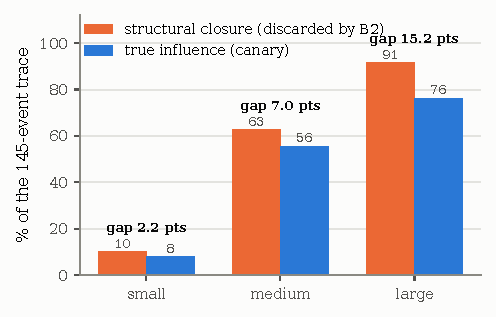
\includegraphics[width=\columnwidth]{figures/fig_exposure_influence.pdf}
\caption{The quantity the method exploits, measured on the testbed. The orange
bar is what reachability-based recovery discards; the blue bar is the fraction a
canary token shows was genuinely affected. The gap is the headroom available to
any influence-aware method, and it widens as contamination grows.}
\label{fig:gap}
\end{figure}

Figure~\ref{fig:gap} shows the measured separation. The gap is $2.2$ points in
the small regime, $7.0$ in the medium and $15.2$ in the large.

\textbf{Interpretation.} The gap is not constant: it grows with the
contaminated fraction. This is the expected consequence of the hub topology ---
the more records are poisoned, the more of the downstream trace becomes
\emph{reachable} from a flagged source, while the number of specialists that
actually \emph{use} a poisoned record grows more slowly. The gap is an upper
bound on what any influence-aware method can recover, not a result in itself.

\subsection{Main result}

\begin{table}[t]
\centering
\caption{Work preserved, 15 runs with 15 distinct attack placements. $\Delta$ is
the paired per-run difference against \btwo{}, in percentage points.}
\label{tab:main}
\footnotesize
\setlength{\tabcolsep}{3.5pt}
\begin{tabular}{lrrrrrrr}
\toprule
\textbf{Regime} & \textbf{$f$ true} & \bzero{} & \bone{} & \btwo{} &
\textbf{\sys{}} & \textbf{$\Delta$} & \textbf{W/T/L}\\
\midrule
small  & 6.2--9.0\%   & 0.0\% & 89.9\% & 89.9\% & 72.6\% & $-17.38$ & 2/2/\textbf{1}\\
medium & 51.7--57.2\% & 0.0\% & 38.1\% & 37.4\% & \textbf{44.4\%} & $+7.03$ & \textbf{5}/0/0\\
large  & 75.2--77.2\% & 0.0\% & 9.2\%  & 8.6\%  & \textbf{23.7\%} & $+15.17$ & \textbf{5}/0/0\\
\bottomrule
\end{tabular}
\end{table}

\begin{figure}[t]
\centering
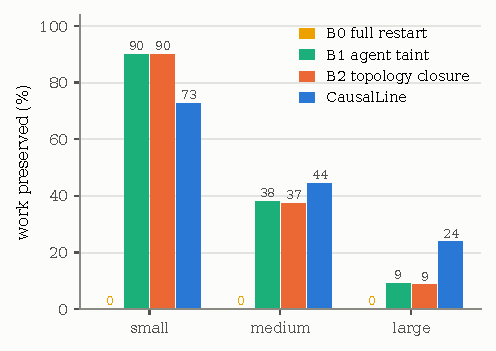
\includegraphics[width=\columnwidth]{figures/fig_preserved.pdf}
\caption{Work preserved by each method, averaged over five distinct attack
placements per regime. \bzero{} preserves nothing by definition. The advantage
of influence-aware recovery over the closure is largest where the closure
performs worst, and is absent where the closure already performs well.}
\label{fig:preserved}
\end{figure}

Table~\ref{tab:main} and Figure~\ref{fig:preserved} give the main result. The
standard deviation of the paired difference is $1.85$ points in the medium
regime and $1.54$ in the large, against $41.97$ in the small.

\textbf{Observed result.} \sys{} wins all five runs in the medium and large
regimes and loses one of five in the small regime. We deliberately report no
aggregate across regimes: pooling the fifteen gives $+1.61$ points with a
standard deviation of $26.64$, a figure that averages three regimes whose
effects have opposite signs and is dominated by a single run. It describes no
situation an operator is ever in.

\textbf{Interpretation.} The result is a boundary, not a uniform win. Where the
poisoned set is large, the reachability closure collapses toward discarding
everything --- \btwo{} retains $8.6\%$ --- and influence analysis still finds
roughly a quarter of the trace to keep. Where the attack enters late, the
closure is already nearly optimal at $89.9\%$ and there is almost nothing left
to recover; \sys{} nonetheless pays the full attribution cost and then verifies,
and when verification fails twice the ladder surrenders the entire gain. The
practical reading is a deployment rule: \emph{where the topology closure is
already near-optimal, this method should not be used}.

The single loss is worth stating precisely. In that run selective replay failed
verification, agent restart failed verification, and recovery delivered
correctly at full restart, preserving $0\%$ against \btwo{}'s $92.4\%$. The
baselines are never charged for this, because they ship unverified recoveries;
in these five runs they happened to be correct.

\subsection{Safety}

\begin{table}[t]
\centering
\caption{Safety measures over all 15 runs and all four methods.}
\label{tab:safety}
\footnotesize
\begin{tabular}{lrrr}
\toprule
\textbf{Quantity} & \textbf{small} & \textbf{medium} & \textbf{large}\\
\midrule
Unsafe preservations (all methods) & 0 & 0 & 0\\
Contamination escapes              & 0 & 0 & 0\\
Payload landed                     & 5/5 & 3/5 & 5/5\\
Recall                             & 1.0 & 1.0 & 1.0\\
Final task correct                 & 5/5 & 5/5 & 5/5\\
Degraded agents                    & 0 & 0 & 0\\
\bottomrule
\end{tabular}
\end{table}

Table~\ref{tab:safety} is the result the project would be withdrawn over. No
method preserved a contaminated event in any run, contamination never escaped
the structural closure, and all fifteen runs produced a correct final result.
On the deterministic scripted matrix --- $96$ cells $\times\,30$ repetitions
under four detectors including a blind control that flags nothing --- \sys{}
recorded unsafe preservations in $0$ of its $24$ cells.

\textbf{Caveat.} Two of the fifteen runs did not land their payload, so for
those runs a zero unsafe count is arithmetic rather than evidence; they are
included because excluding runs on an outcome would be selection, and flagged
because they should be weighted differently. The decoupling of structural
divergence from outcome corruption reported by~\cite{tracelevel2026} is the
same hazard, and is why landing is reported separately from task success.

\subsection{Economic analysis}

\begin{table}[t]
\centering
\caption{Mean recovery cost per run, in tokens. \sys{} pays analysis plus
replay; the baselines pay replay only.}
\label{tab:cost}
\footnotesize
\begin{tabular}{lrrrr}
\toprule
\textbf{Regime} & \textbf{\btwo{}} & \textbf{\sys{} anal.} &
\textbf{\sys{} total} & \textbf{vs \bzero{}}\\
\midrule
small  & 1\,595 & 16\,312 & 19\,598 & $1.8\times$\\
medium & 7\,975 & 15\,796 & 23\,771 & $2.2\times$\\
large  & 9\,772 & 15\,911 & 25\,683 & $2.5\times$\\
\bottomrule
\end{tabular}
\end{table}

\begin{figure}[t]
\centering
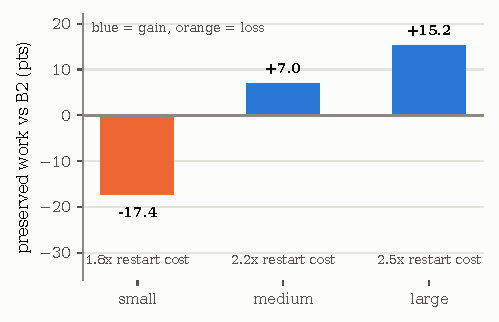
\includegraphics[width=\columnwidth]{figures/fig_cost.pdf}
\caption{What the additional tokens buy. The bar is the paired difference in
preserved work against the closure baseline; the annotation below each bar is
the total cost as a multiple of simply re-running the whole workflow. The
method is more expensive than restart in every regime, and the trade improves
as contamination grows.}
\label{fig:cost}
\end{figure}

Table~\ref{tab:cost} and Figure~\ref{fig:cost} state the cost plainly:
\emph{\sys{} is more expensive in tokens than every baseline, including full
restart}, at $1.8\times$ to $2.5\times$ the cost of re-running the workflow.
Attribution rather than replay dominates, accounting for $62$--$83\%$ of the
total.

\textbf{Interpretation.} If tokens are the only cost and the workflow can
simply be re-run, restart is the correct choice and this method is not. The
case for it is the case where that assumption fails: work with external side
effects cannot be undone by restarting, only repeated; re-execution of an LLM
pipeline is not idempotent, so a restart produces a different run that may be
worse; and in our measurements wall-clock time was dominated by provider rate
limiting rather than token count. These are stated as the conditions under
which the trade is favourable, not as measured results --- the testbed's work is
replayable by construction, which is what makes it measurable at all.

\subsection{Escalation behaviour}

Across the fifteen runs, twelve recoveries were delivered at the selective
scope, two at agent restart and one at full restart. Three runs escalated at
least once, with four verification failures in total; the escalation budget was
never exhausted and no provider degradation occurred.
This confirms that restart functions as a fallback rather than as the primary
action, which is the property the verification layer exists to provide.

\subsection{A defect that presented as an improvement}
\label{sec:defect}

During the campaign the large regime initially reported \sys{} preserving
$31.7\%$ against \btwo{}'s $14.5\%$ --- a $+17.2$-point improvement --- together
with \emph{five unsafe preservations}. All five were \texttt{memory\_read}
events whose stored output contained the poisoned policy text.

The cause was a missing relation rather than a wrong verdict. The event that
retrieves a source stores that source's text in its own output, but the source
does not exist when the event is logged, so it was never in that event's
exposures, so no verdict was ever written for the pair and the propagation walk
never considered it. Adding the ingestion relation closed the gap; the regime
then read $14.5\%$ with zero unsafe preservations. \emph{The entire apparent
improvement was the defect.}

Two lessons were recorded. First, work preserved and unsafe preservations are
not independent: any mechanism that preserves more is mechanically a candidate
for preserving something it should not, so the two must be read together.
Second, the defect was found by observed ground truth --- a canary in an output
--- and would not have been found by construction-based ground truth, which by
construction holds that a source did not influence the event that produced it.

\subsection{Threats to validity}

\begin{enumerate}
\item \textbf{Five workloads per regime.} Five draws support descriptive
statistics and a sign count, not a distributional claim about how often the
benefit appears. The small regime's standard deviation of $41.97$ shows that
five draws are few when the outcome is bimodal between "selective succeeded"
and "escalated to restart".
\item \textbf{One topology.} Nothing here says how the result behaves as hub
fan-out, stage depth or provider mix change.
\item \textbf{Oracle detector.} We measure recovery after detection and say
nothing about detection quality.
\item \textbf{A copy task.} Each agent moves a short code. This was chosen so
that capability failures of a small local model do not masquerade as recovery
failures, and it means nothing here demonstrates recovery on tasks with
branching control flow or side-effecting tools.
\item \textbf{No significance testing.} None is reported and none would be
meaningful at this sample size.
\item \textbf{The propagation rule is not proved complete.} It is measured
(zero escapes in all runs) and checkable at run time, and it has already been
incomplete once (Section~\ref{sec:defect}).
\item \textbf{Band compliance.} The medium regime's measured contaminated
fraction lies in $51.7$--$57.2\%$ against an intended $25$--$50\%$ band. This is
a property of the topology --- any Stage~A poisoning reaches the hub, and
everything downstream of the hub is roughly half the trace --- and is reported
rather than corrected; no seed was rejected for producing an inconvenient value.
\end{enumerate}

%==============================================================================
\section{Conclusion and Future Directions}
\label{sec:concl}

This project addressed recovery after a confirmed prompt-injection compromise in
a multi-agent LLM system: given a detector's verdict, deciding which completed
work must be recomputed. We implemented \sys{}, which records provenance during
execution, estimates per-pair influence under an asymmetric evidence discipline,
propagates contamination along three recorded relations rather than
reachability, replays only affected events while splicing the rest byte-exactly,
and verifies the recovered run before accepting it, escalating to restart on
failure.

\textbf{Key findings.} On a 56-agent, three-provider workflow with fifteen
distinct attack placements, the method preserved $7.0$ and $15.2$ percentage
points more correct work than the topology-closure baseline in the two heavier
contamination regimes, and lost $17.4$ points in the light regime where the
baseline is already near-optimal. Safety held throughout: zero unsafe
preservations, zero contamination escapes and recall $1.0$ across all fifteen
runs, and zero unsafe preservations across $24$ scripted cells at $30$
repetitions under four detectors. The method costs $1.8\times$ to $2.5\times$ a
full restart in tokens, so it is not a cost optimisation.

\textbf{Current limitations.} The evaluation covers one topology, one detector
model, a deliberately simple task, and five workloads per regime. The
propagation rule is validated empirically rather than proved complete.

\textbf{Future directions}, in the order we judge most useful:
\begin{enumerate}
\item A task with branching control flow and side-effecting tools, which is the
single largest gap between the testbed and a deployed pipeline.
\item A larger campaign varying hub fan-out and stage depth, to test whether the
advantage scales with topology as the current data suggests.
\item An adversarial pass aimed specifically at finding a fourth propagation
relation, rather than relying on the one defect found incidentally.
\item Replacing the oracle detector with a real one, to measure how recovery
quality degrades as the flagged set becomes imperfect.
\item Reducing attribution cost, which dominates the economics; prior
measurement in this project found a large fraction of self-report calls land
outside the contaminated closure and cannot change the outcome.
\item Extension of this work into a conference submission, for which the first
two items are prerequisites.
\end{enumerate}

%==============================================================================
\appendix
\section*{Appendix: Reproduction}

Every table and figure in Section~\ref{sec:exp} is regenerated from committed
result files by the following commands, run from the repository root.

\begin{table}[h]
\centering
\footnotesize
\begin{tabular}{ll}
\toprule
\textbf{Artefact} & \textbf{Command}\\
\midrule
Main campaign & \texttt{python -m src.eval.mixed\_validation}\\
              & \texttt{\ \ --seeds 5 --vary-placement}\\
Result tables & \texttt{python -m src.eval.}\\
              & \texttt{\ \ mixed\_validation\_report}\\
Scripted matrix & \texttt{python -m src.eval.campaign --reps 30}\\
Figures & \texttt{python diagrams/make\_figures.py}\\
Test suite & \texttt{python -m unittest discover -s tests}\\
\bottomrule
\end{tabular}
\end{table}

The campaign writes one JSON file per run, is resumable, and skips runs already
on disk, so an interrupted campaign is continued rather than restarted. Figures
are produced from \texttt{diagrams/topology.json} and
\texttt{diagrams/results.json}, which are themselves derived from an executed
trace and from the committed result files respectively.

%==============================================================================
\section*{Acknowledgment}

The authors thank the project supervisor for guidance on experimental design,
and in particular for the insistence that negative results and corrections be
reported rather than removed.

%==============================================================================
% References are listed inline rather than through BibTeX, so the document
% builds in a single pdflatex pass with no .bst file. `references.bib` is kept
% alongside this file and carries the same 15 entries for anyone converting the
% report to a BibTeX-based template later.
\begin{thebibliography}{99}
\footnotesize

\bibitem{greshake2023}
K. Greshake, S. Abdelnabi, S. Mishra, C. Endres, T. Holz, and M. Fritz,
``Not what you've signed up for: Compromising real-world LLM-integrated
applications with indirect prompt injection,'' in \emph{Proc. 16th ACM Workshop
on Artificial Intelligence and Security (AISec)}, 2023, pp. 79--90.

\bibitem{perez2022}
F. Perez and I. Ribeiro, ``Ignore previous prompt: Attack techniques for
language models,'' in \emph{NeurIPS Workshop on ML Safety}, 2022.

\bibitem{liu2024}
Y. Liu, Y. Jia, R. Geng, J. Jia, and N. Z. Gong, ``Formalizing and benchmarking
prompt injection attacks and defenses,'' in \emph{Proc. 33rd USENIX Security
Symposium}, 2024.

\bibitem{chen2024}
S. Chen, J. Piet, C. Sitawarin, and D. Wagner, ``StruQ: Defending against
prompt injection with structured queries,'' in \emph{Proc. 33rd USENIX Security
Symposium}, 2024.

\bibitem{neurotaint2026}
Y. Cai, W. Tang, C. Wen, and S. Qin, ``Ghost in the agent: Redefining
information flow tracking for LLM agents,'' \emph{arXiv:2604.23374}, 2026.

\bibitem{granularity2026}
L. Fan, Z. Li, Y. Tian, Y. Wang, R. Li, and X. Wang, ``The granularity mismatch
in agent security: Argument-level provenance solves enforcement and isolates
the LLM reasoning bottleneck,'' \emph{arXiv:2605.11039}, 2026.

\bibitem{car2026}
J. Shah, ``Causal agent replay: Counterfactual attribution for LLM-agent
failures,'' \emph{arXiv:2606.08275}, 2026.

\bibitem{causalflow2026}
A. Bonagiri, D. Borkar, G. J. Anderias, S. Rafatirad, and H. Homayoun,
``CausalFlow: Causal attribution and counterfactual repair for LLM agent
failures,'' \emph{arXiv:2605.25338}, 2026.

\bibitem{tracelevel2026}
A. Mazhar, H. Suri, and S. Galhotra, ``Trace-level analysis of information
contamination in multi-agent systems,'' \emph{arXiv:2604.27586}, 2026.

\bibitem{dover2026}
M. Ma, J. Zhang, F. Yang, Y. Kang, Q. Lin, S. Rajmohan, and D. Zhang, ``DoVer:
Intervention-driven auto debugging for LLM multi-agent systems,''
\emph{arXiv:2512.06749}, 2026.

\bibitem{zeroreplay2026}
D. H. Kang, H. Cha, and D. Weon, ``Knowledge-based zero-replay debugging of
multi-agent LLM traces,'' \emph{arXiv:2606.14805}, 2026.

\bibitem{trustsurvey2026}
Y. Wang, J. Zhang, Z. Wu \emph{et al.}, ``From agent traces to trust: A survey
of evidence tracing and execution provenance in LLM agents,''
\emph{arXiv:2606.04990}, 2026.

\bibitem{newsome2005}
J. Newsome and D. Song, ``Dynamic taint analysis for automatic detection,
analysis, and signature generation of exploits on commodity software,'' in
\emph{Proc. Network and Distributed System Security Symp. (NDSS)}, 2005.

\bibitem{king2003}
S. T. King and P. M. Chen, ``Backtracking intrusions,'' in \emph{Proc. 19th ACM
Symp. on Operating Systems Principles (SOSP)}, 2003, pp. 223--236.

\bibitem{elnozahy2002}
E. N. Elnozahy, L. Alvisi, Y.-M. Wang, and D. B. Johnson, ``A survey of
rollback-recovery protocols in message-passing systems,'' \emph{ACM Computing
Surveys}, vol. 34, no. 3, pp. 375--408, 2002.

\end{thebibliography}

\end{document}
